\documentclass{minimal}
\usepackage{amsmath}
\usepackage{ctex}
\usepackage{graphicx}
\begin{document}
关于箱体的组成部分有:箱体、箱须和离群值,其中,箱体主要由第一四分位数、中位数和第三四分位数组成,箱须又分为上箱须和下箱须。下面,介绍一下这些组成部分的含义和计算方法。上箱须和下箱须长度的确定方法是在绘制箱线图的原始数据集 Data 中分别寻找不大于 $Q_3+whis\times IQR$ 的最大值 $value{max}$ 和不小于 $Q_1-whis\times IQR$ 的最小值 $value_{min}$,其中 $Q_1$ 和 $Q_3$ 分别是第一四分位数和第三四分位数,whis 是关键字参数 whis 的参数值(\verb|plt.boxplot()|),IQR(IQR 是 Inter-Quartile Range 的缩写)是四分位差,计算方法是 $IQR=Q_3-Q_1$。离群值 Outlier 的判断标准是 $value<(Q_1-whis\times IQR)$ 或者 $value>(Q_3+whis\times IQR)$,其中,value 是数据集 Data 中的数据点。下面,为了清楚地掌握箱线图的结构组成,如图所示的示意图来阐述箱线图的各个组成元素。

\begin{center}
    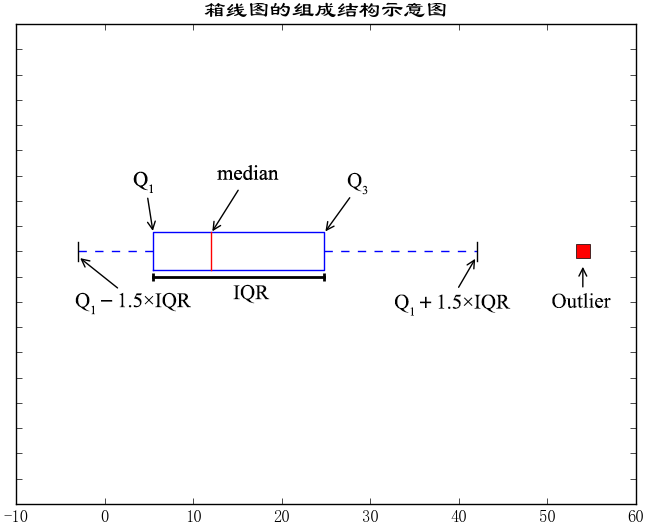
\includegraphics[width=.7\textwidth]{./fig3-22.png}
\end{center}
\end{document}